\chapter{Studies on the $\mathbf{Z(\rightarrow\nu\bar{\nu})}$+jets background}
    \label{app:ClosureTestZnunu}

The main irreducible background in the analysis, $\znn$, is normalized with the same factor (see Section~\ref{sec:Fit}) as the $\wmn$+jets background.
This irreducible background could also have been normalized using the same normalization as the $\zmm$+jets process.
This appendix presents additional studies with the aim to:

\begin{itemize}
\item Confirm the validity of the approach adopted, in which the irreducible $\znn$ and $\wmn$+jets processes are normalized with the same normalization factor.

\item Establish to which extent $\wmn$+jets and/or $\zmm$+jets processes can be used to determine the $\znn$ normalization in terms of their shape.

\item Consider the impact of higher order electroweak corrections, affecting differently the $W$+jets and the $Z$+jets processes.
\end{itemize}

Figure~\ref{fig:ClosurePlotNormalized1} compares the shape of different particle level and reconstructed quantities in the MC simulations between for $\wmn$+jets, $Z/\gamma^{\ast}(\rightarrow \mu^{+}\mu^{-})$+jets, and $\znn$ processes.
In this figure, the selection criteria for the region M1 are applied, except for those requirements on the leptons.
This study has also been done separately for the other signal regions. 
The ratio of $\wmn$+jets to $\znn$  is rather flat in all distributions and contained within a $\pm 3\%$ band.
This is also valid for the $\zmm$+jets process although in this case, statistical uncertainties are large.

%
% --- plots normalized
%

\begin{figure}
\begin{center}
\mbox{
  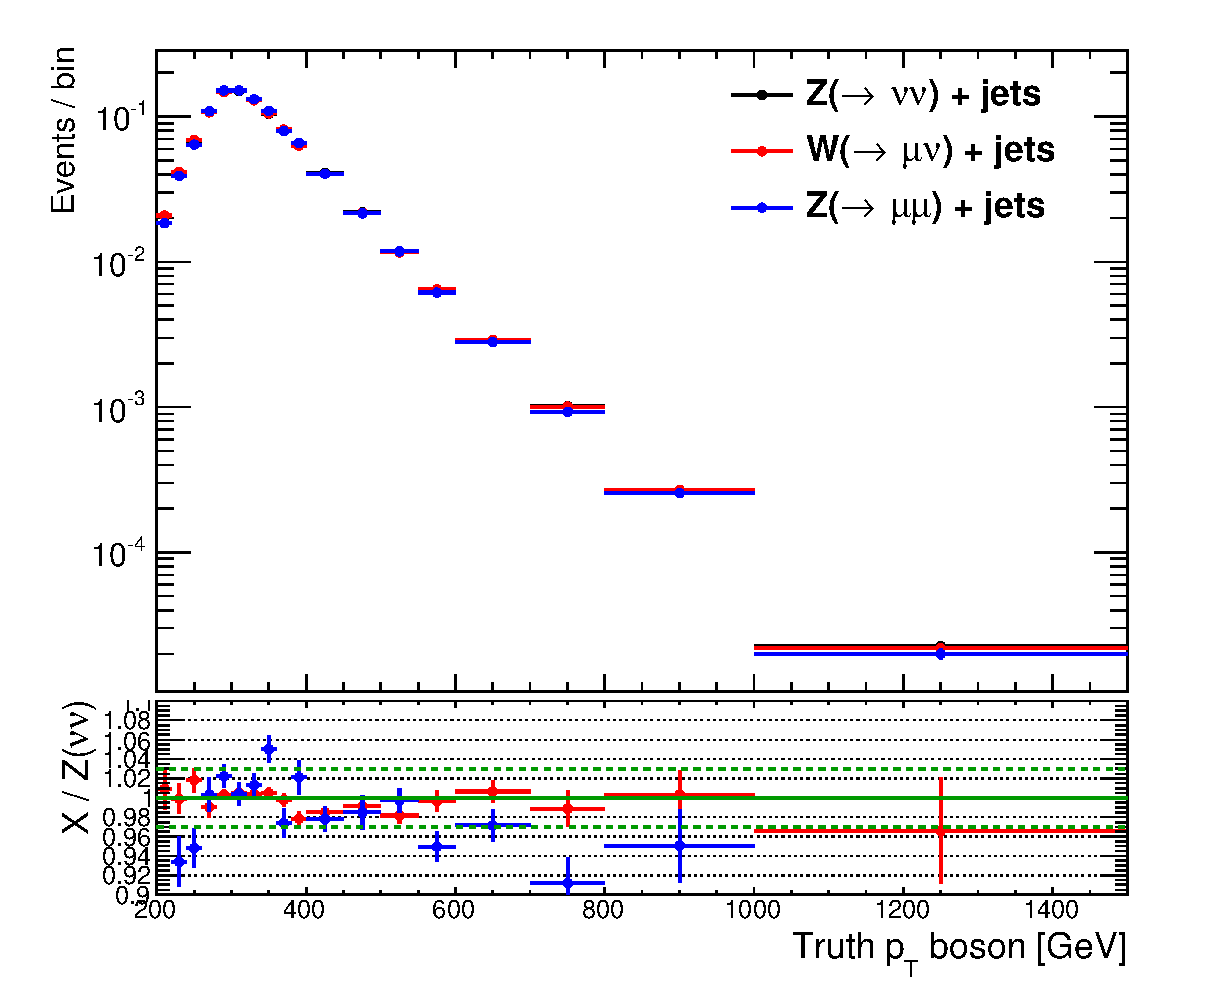
\includegraphics[width=0.49\textwidth]{Appendix_ClosureTestZnunu/Figures/compareNormalized_bosonVec_truth_pt_A6_Nom.eps}
  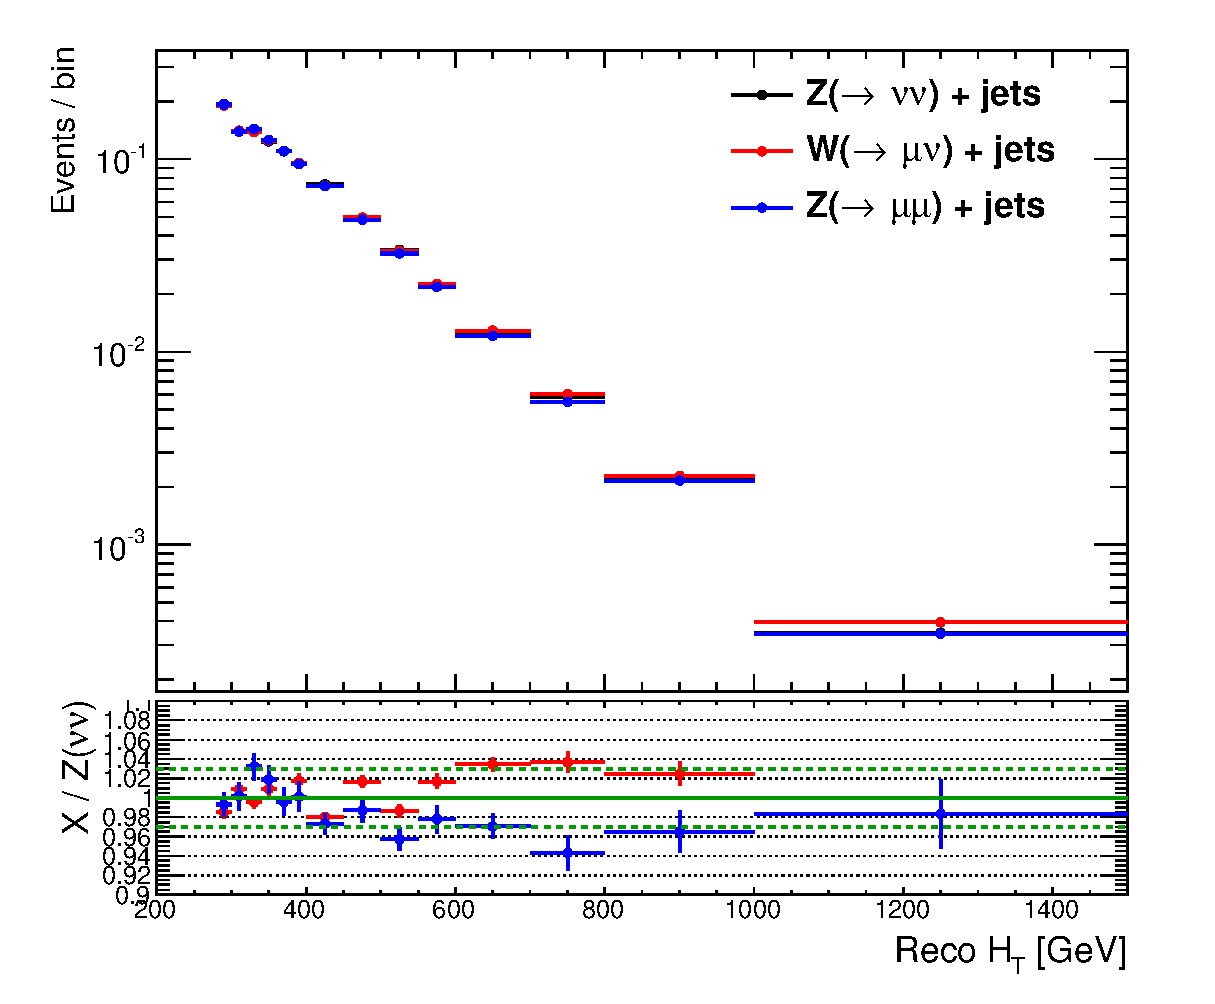
\includegraphics[width=0.49\textwidth]{Appendix_ClosureTestZnunu/Figures/compareNormalized_HT_A6_Nom.eps}
}
\mbox{
  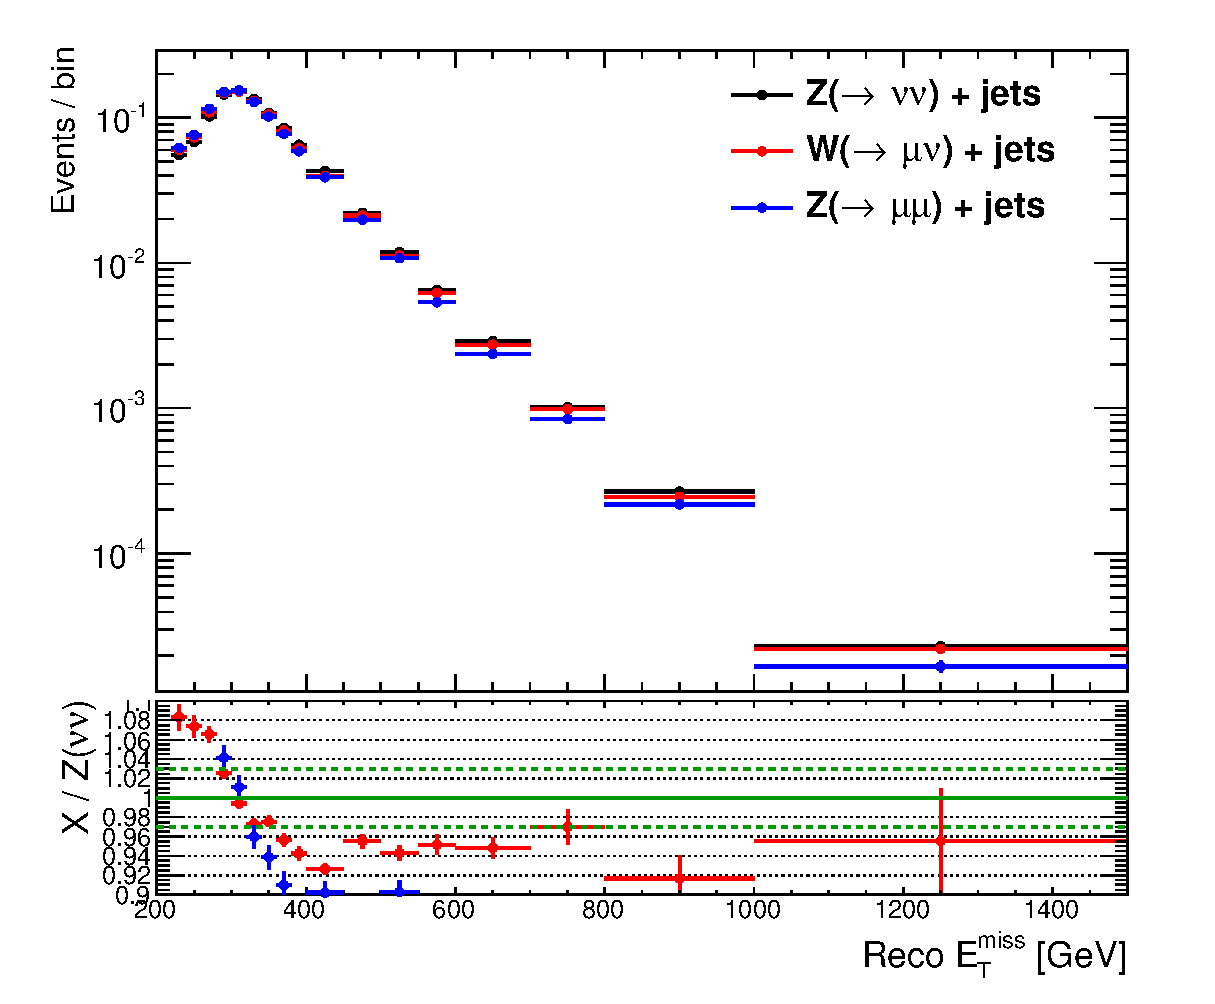
\includegraphics[width=0.49\textwidth]{Appendix_ClosureTestZnunu/Figures/compareNormalized_met_A6_Nom.eps}
  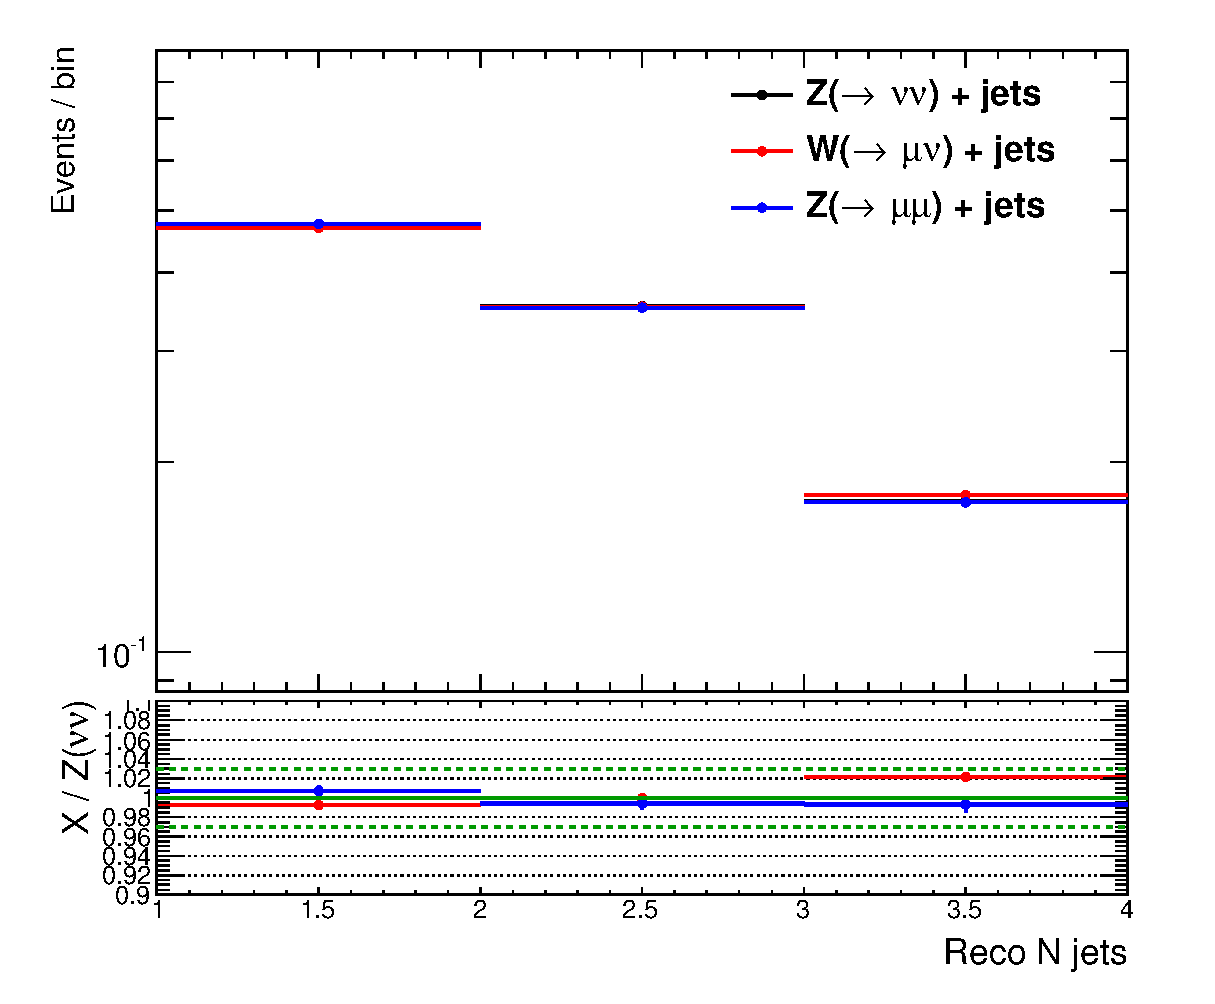
\includegraphics[width=0.49\textwidth]{Appendix_ClosureTestZnunu/Figures/compareNormalized_n_jets_A6_Nom.eps}
}
\mbox{
  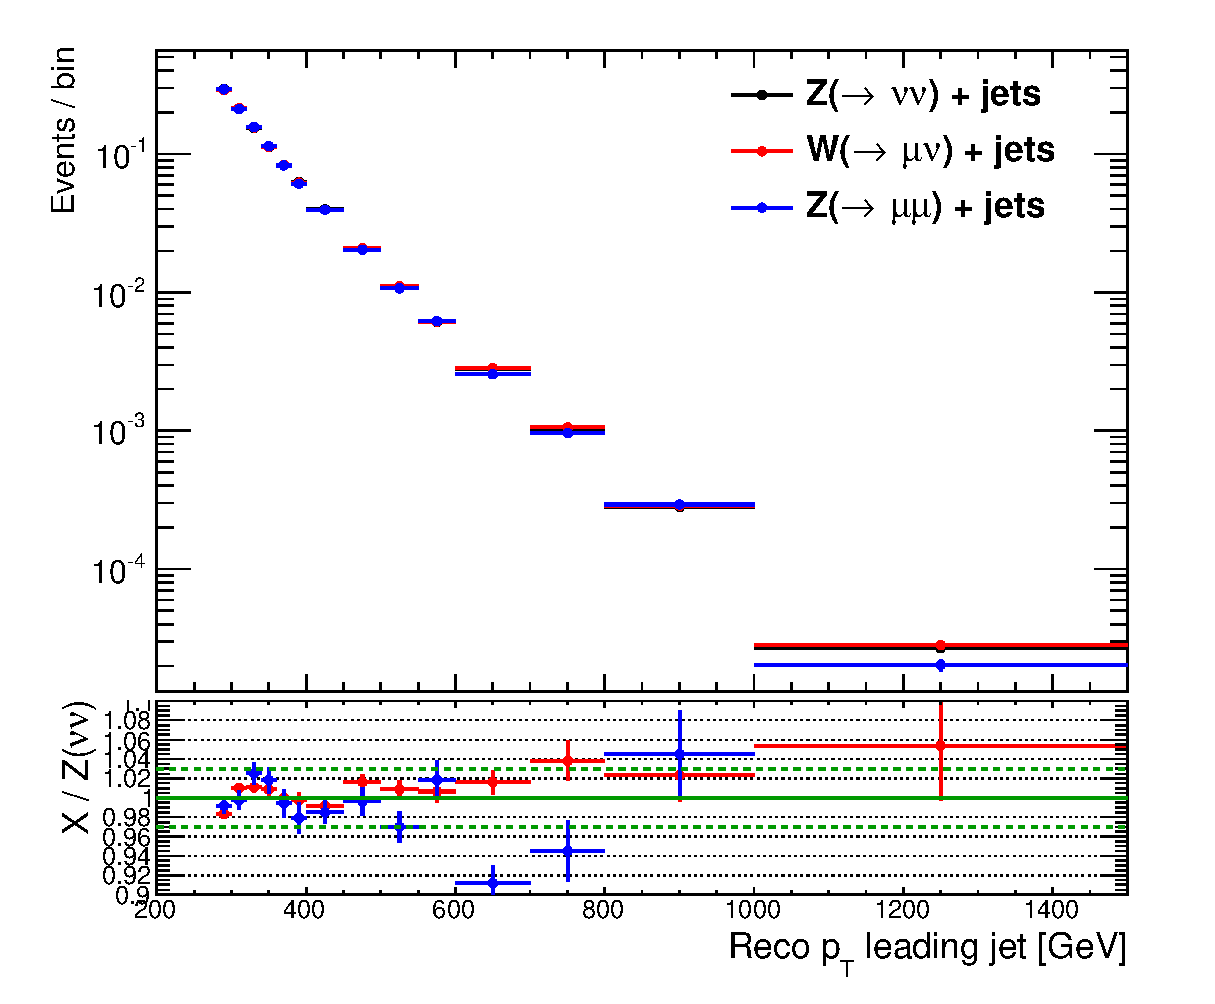
\includegraphics[width=0.49\textwidth]{Appendix_ClosureTestZnunu/Figures/compareNormalized_pt1_A6_Nom.eps}
  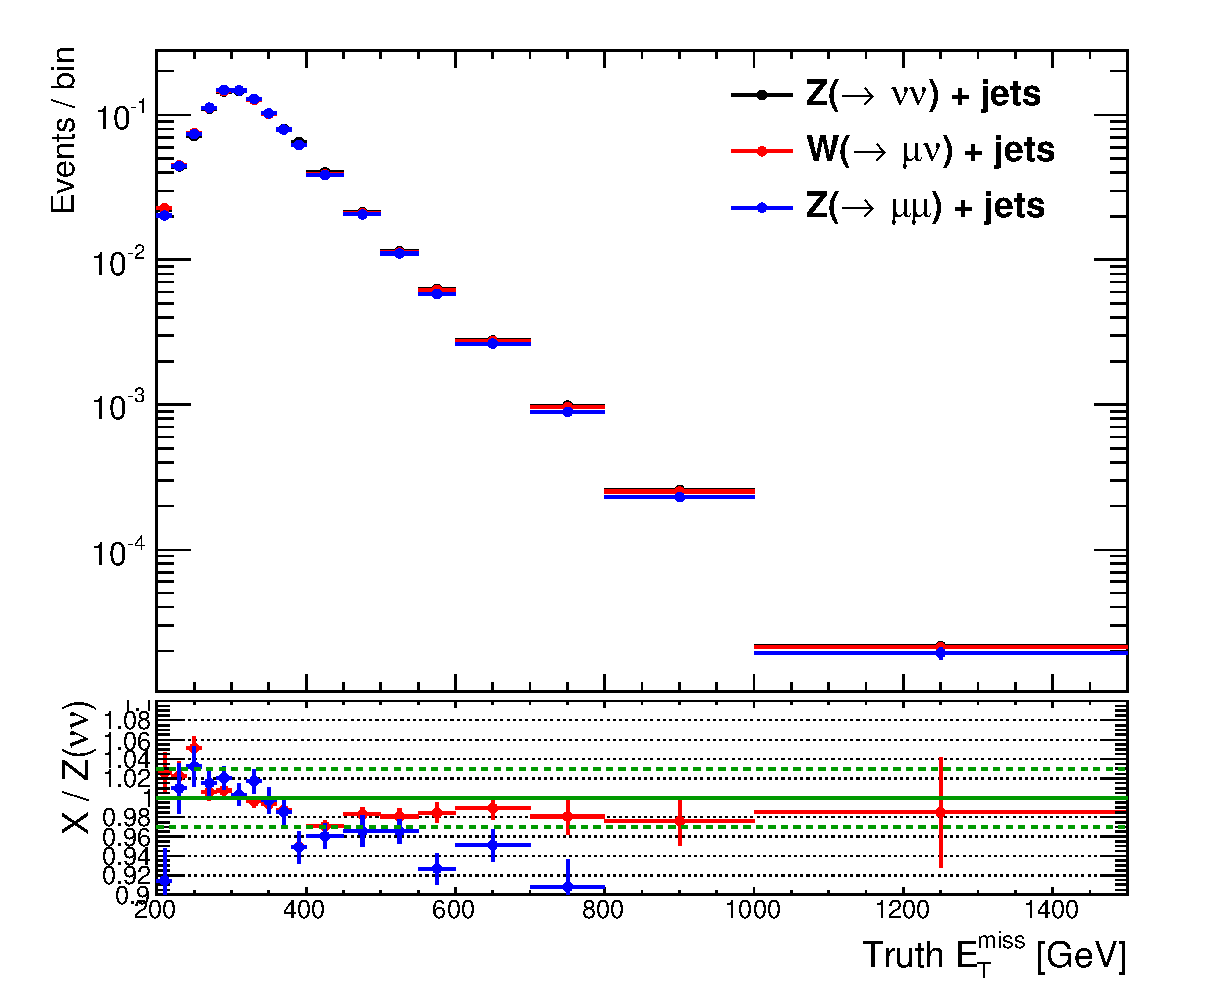
\includegraphics[width=0.49\textwidth]{Appendix_ClosureTestZnunu/Figures/compareNormalized_truth_met_A6_Nom.eps}
}
\end{center}
\caption[Comparison of different quantities with the M1 kinematic selection, with no fiducial cuts in the invariant or transverse mass, between $\wmn$+jets, $\zmm$+jets and $\znn$ MC simulations.]{
Comparison of different quantities with the M1 kinematic selection between $\wmn$+jets, $\zmm$+jets and $\znn$ MC simulations.
Comparisons are performed using inclusive $W$ and $Z$ production (no fiducial cuts in the $Z$ invariant mass or the $W$ transverse mass).
}
\label{fig:ClosurePlotNormalized1}
\end{figure}

The requirements in the $\pt$ of the muons, the transverse mass, and the invariant mass, that are used in the definition of the control regions to reconstruct the $W$ and $Z$ bosons, respectively, could affect the $W$+jets to $\znn$ ratio.
For this reason, Figure~\ref{fig:closure5} compares, for the M1 selection, the shape of different particle level and reconstructed quantities in the MC simulated $\znn$, $\wmn$+jets, and $\zmm$+jets processes, after the requirements on the leptons are applied respectively to the $\wmn$+jets and $\zmm$+jets control samples.
This reduces the size of the samples and, in some cases, it further improves the similarities in shape with the $\znn$ process.
Altogether, the shape difference between $\wmn$+jets, $\zmm$+jets and $\znn$ is still contained within a $3\%$ uncertainty band.
As shown in the Figures, the fact that the $\zmm$+jets control region has less events than the $\wmn$+jets control region, supports the use of $\wmn$+jets control region to constrain the irreducible $\znn$ background contribution.

\begin{figure}
\begin{center}
\mbox{
  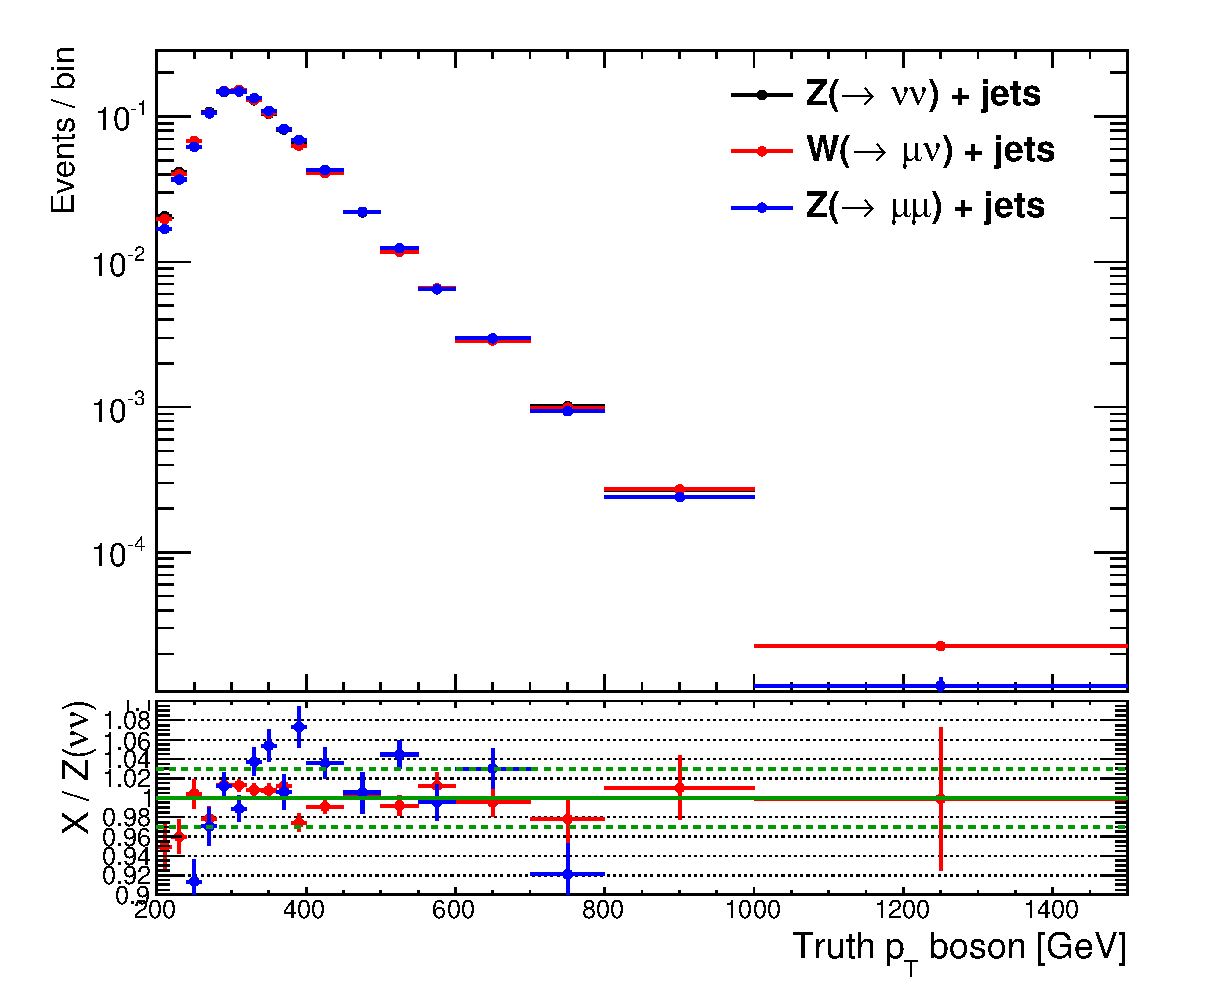
\includegraphics[width=0.49\textwidth]{Appendix_ClosureTestZnunu/Figures/compareNormalized_bosonVec_truth_pt_A6_Nom_CRcutsWZ.eps}
  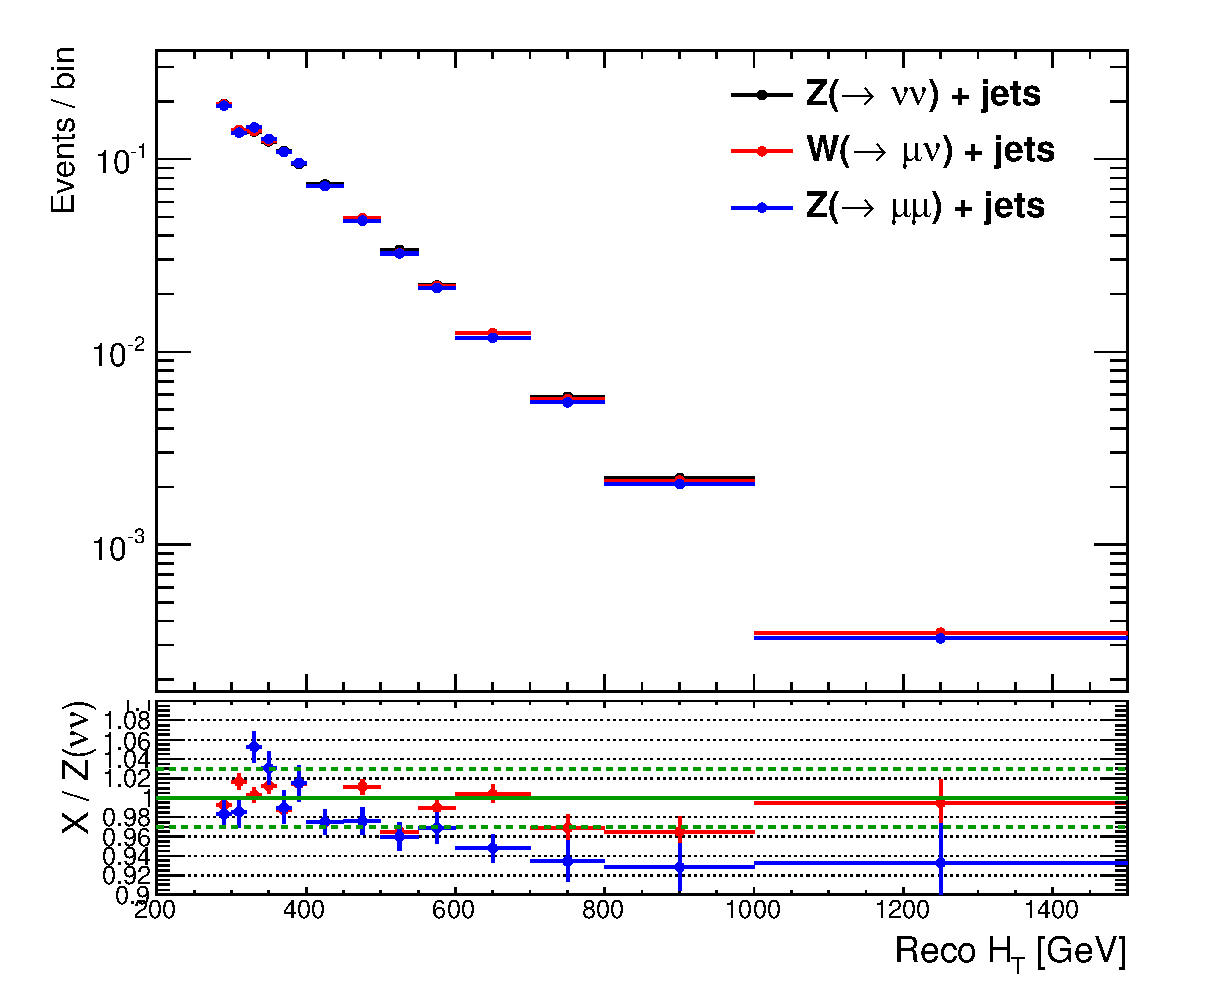
\includegraphics[width=0.49\textwidth]{Appendix_ClosureTestZnunu/Figures/compareNormalized_HT_A6_Nom_CRcutsWZ.eps}
}
\mbox{
  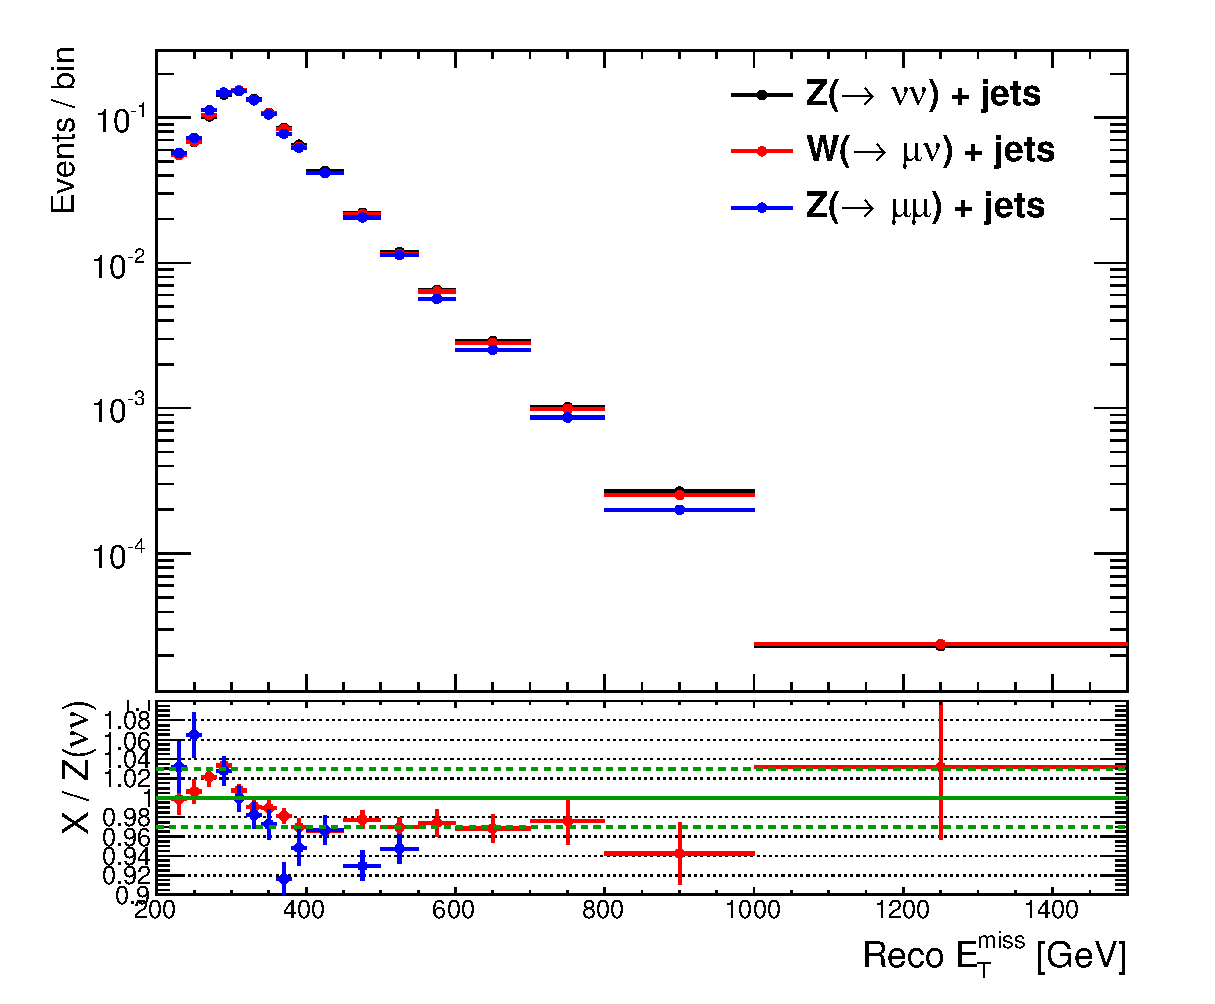
\includegraphics[width=0.49\textwidth]{Appendix_ClosureTestZnunu/Figures/compareNormalized_met_A6_Nom_CRcutsWZ.eps}
  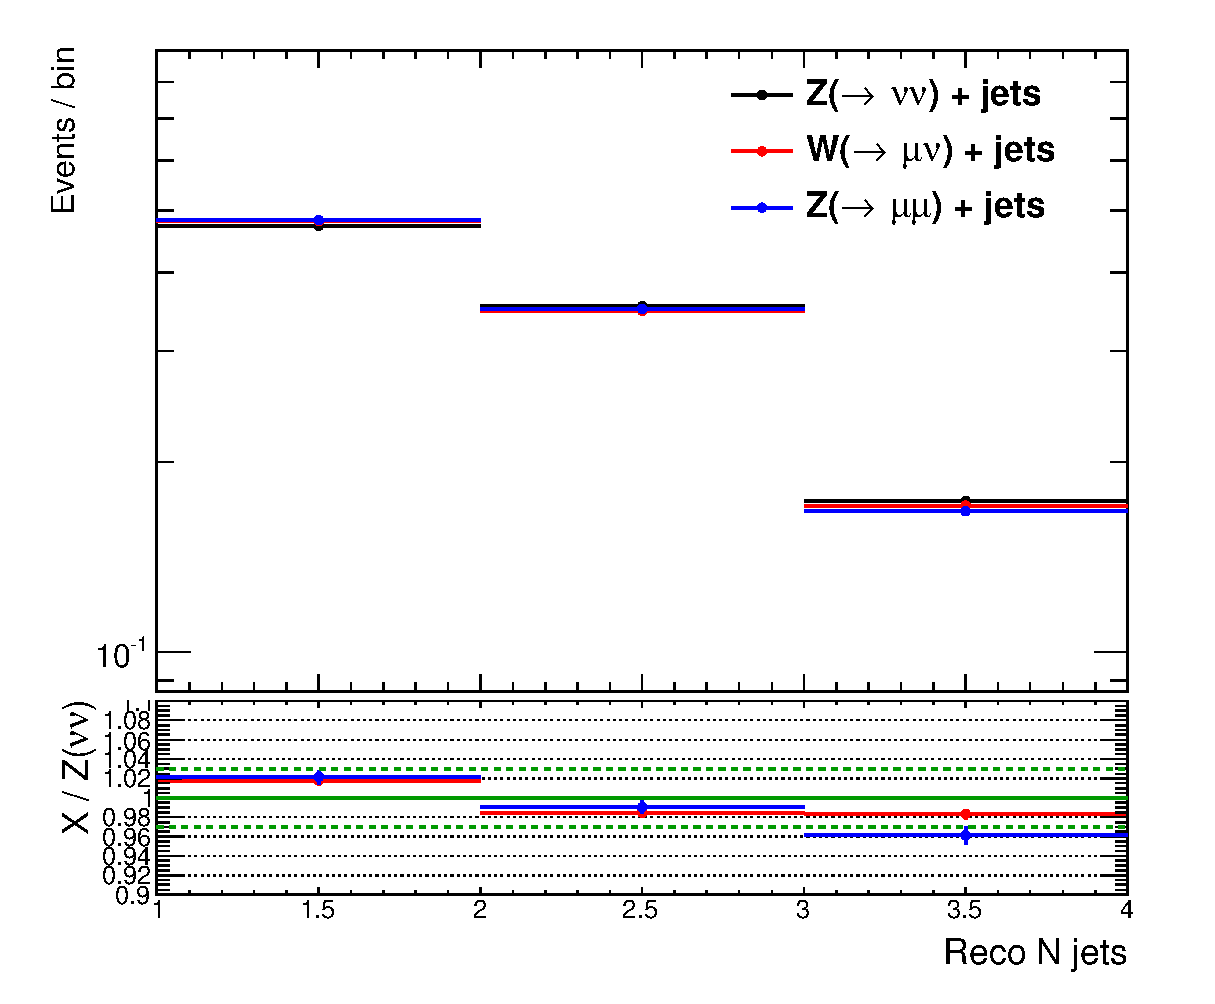
\includegraphics[width=0.49\textwidth]{Appendix_ClosureTestZnunu/Figures/compareNormalized_n_jets_A6_Nom_CRcutsWZ.eps}
}
\mbox{
  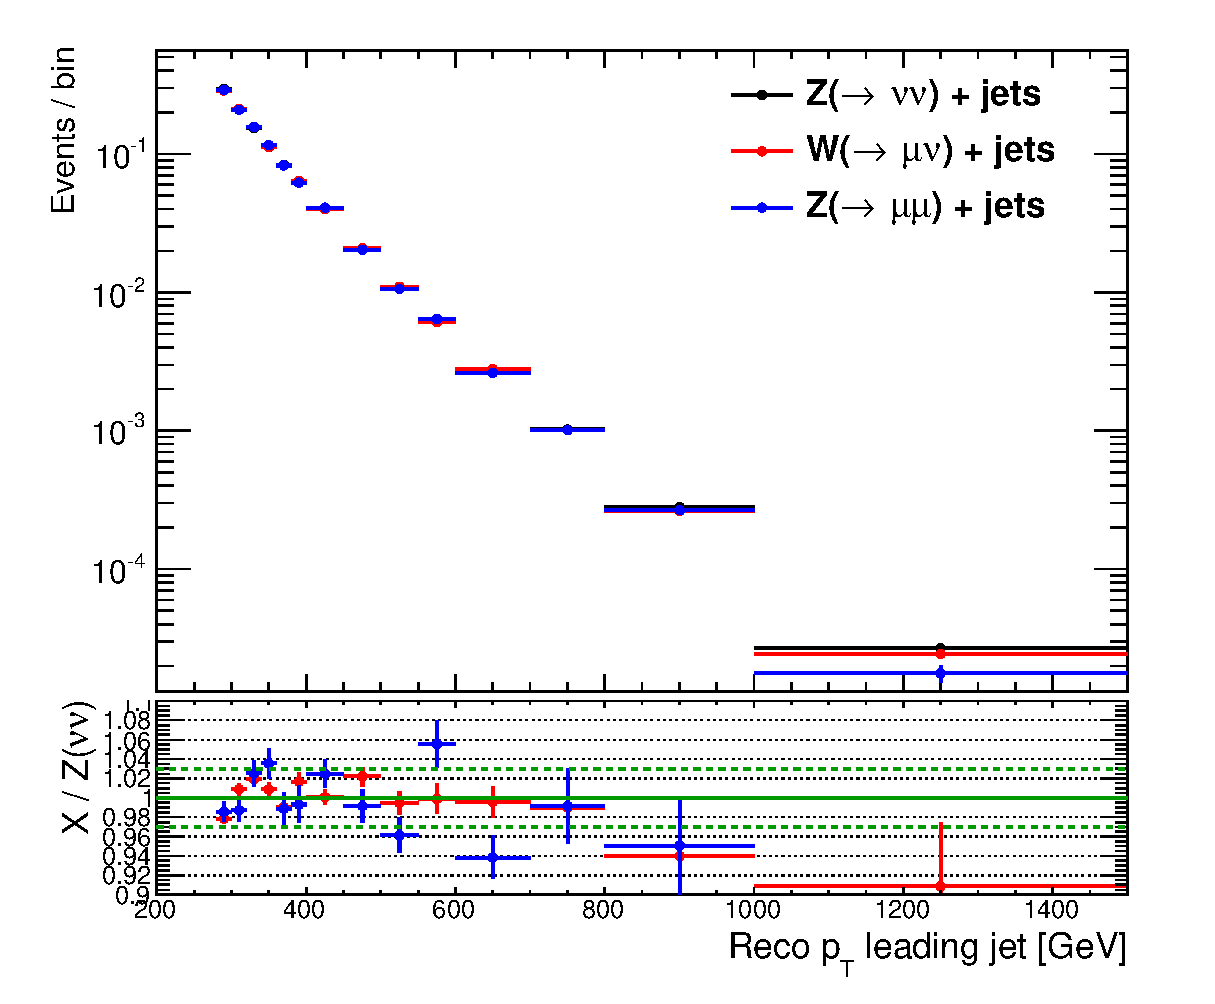
\includegraphics[width=0.49\textwidth]{Appendix_ClosureTestZnunu/Figures/compareNormalized_pt1_A6_Nom_CRcutsWZ.eps}
  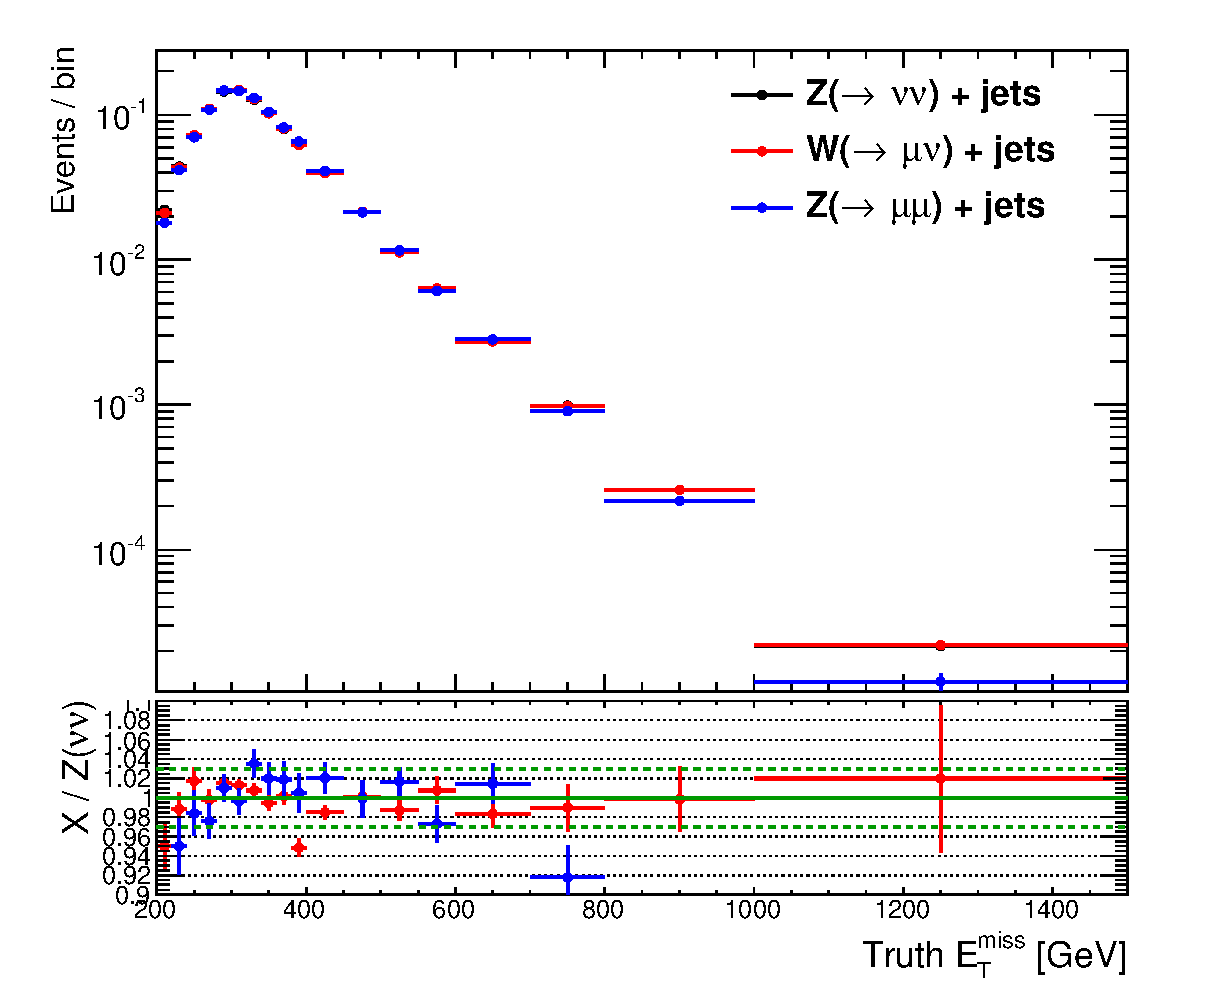
\includegraphics[width=0.49\textwidth]{Appendix_ClosureTestZnunu/Figures/compareNormalized_truth_met_A6_Nom_CRcutsWZ.eps}
}
\end{center}
\caption[Comparison of different quantities with the M1 kinematic selection between $\wmn$+jets, $\zmm$+jets and $\znn$ MC simulations, after the W and Z bosons in the different control regions are reconstructed.]{
Comparison of different quantities with the M1 kinematic selection between $\wmn$+jets, $\zmm$+jets and $\znn$ MC simulations.
Comparisons are performed after the $W$ and $Z$ bosons in the $\wmn$ and $\zmm$ control regions, respectively, are reconstructed in the MC simulated samples.
}
\label{fig:closure5}
\end{figure}

As a further cross check, an additional study is performed comparing different distributions for the $\wmn$+jets and the $\znn$ samples, when now the neutrinos are treated as muons. 
To do that, the $\wmn$+jets ($\znn$) events are required to have muons (neutrinos) with $\pt^{\mu}>\unit[10]{GeV}$ and $|\eta^{\mu}|<2.4$ ($\pt^{\nu}>\unit[10]{GeV}$ and $|\eta^{\nu}|<2.4$), at the particle level.
The result for this study is shown in Figure~\ref{fig:closure8}, and also concludes that the shape difference between $\wmn$+jets and the $\znn$ is still within a 3\% band.
These studies motivate the addition of a 3\% uncertainty on the estimation of the $\znn$ background process.

\begin{figure}
\begin{center}
\mbox{
  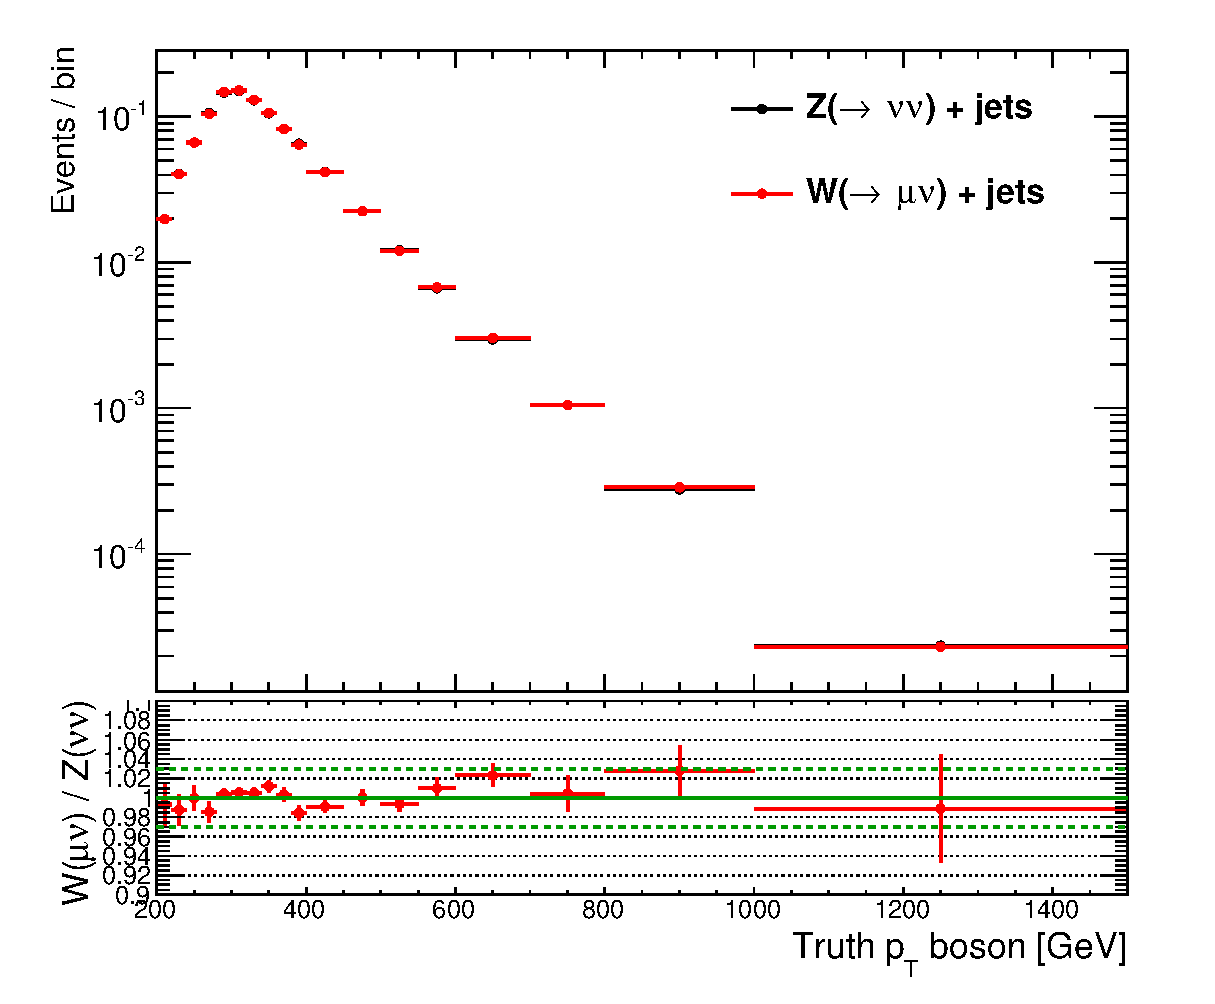
\includegraphics[width=0.49\textwidth]{Appendix_ClosureTestZnunu/Figures/compareNormalized_bosonVec_truth_pt_A6_Nom_CRcutsWZFiducialMu.eps}
  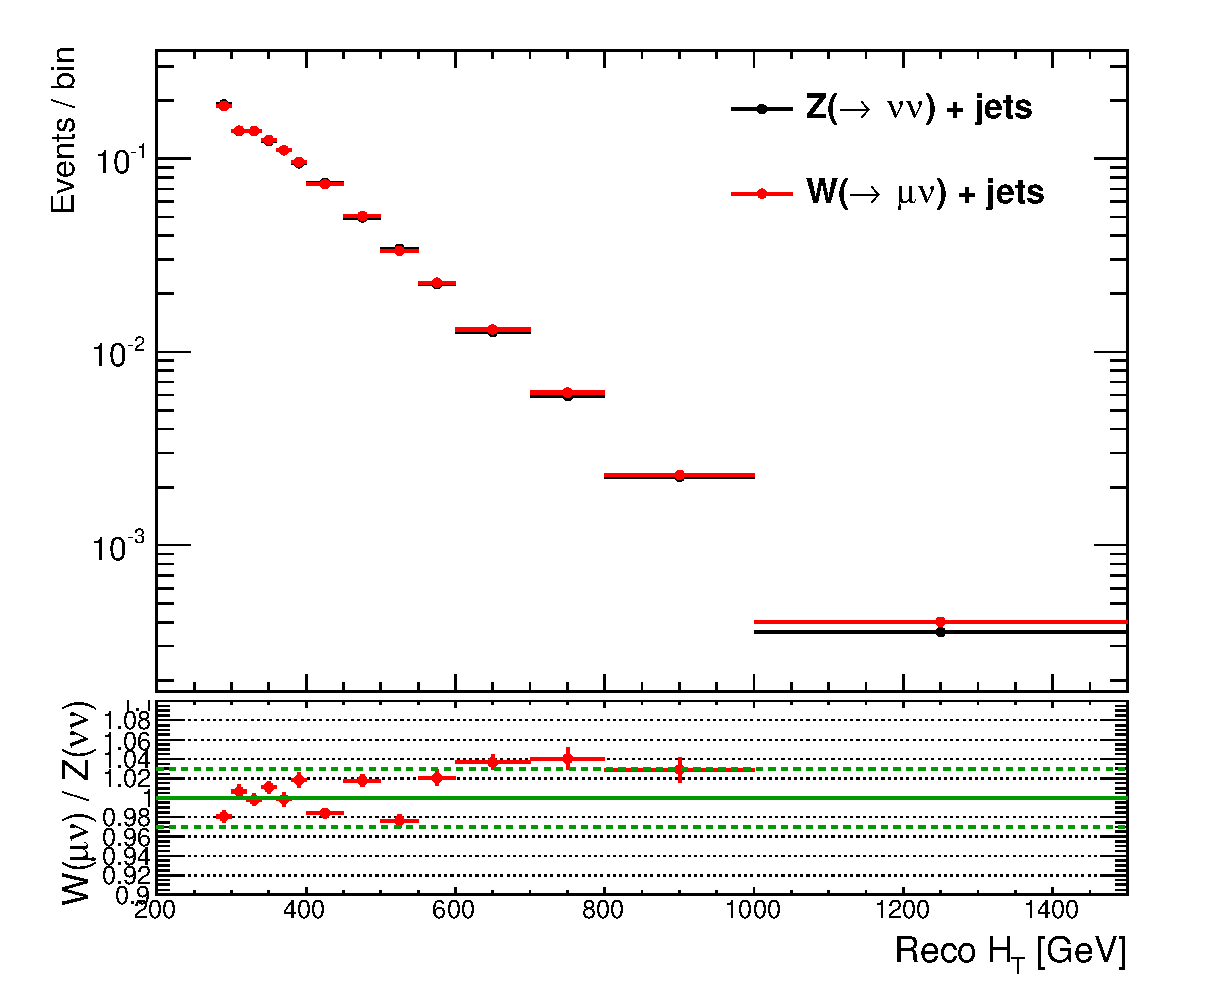
\includegraphics[width=0.49\textwidth]{Appendix_ClosureTestZnunu/Figures/compareNormalized_HT_A6_Nom_CRcutsWZFiducialMu.eps}
}                                                                          
\mbox{                                                                     
  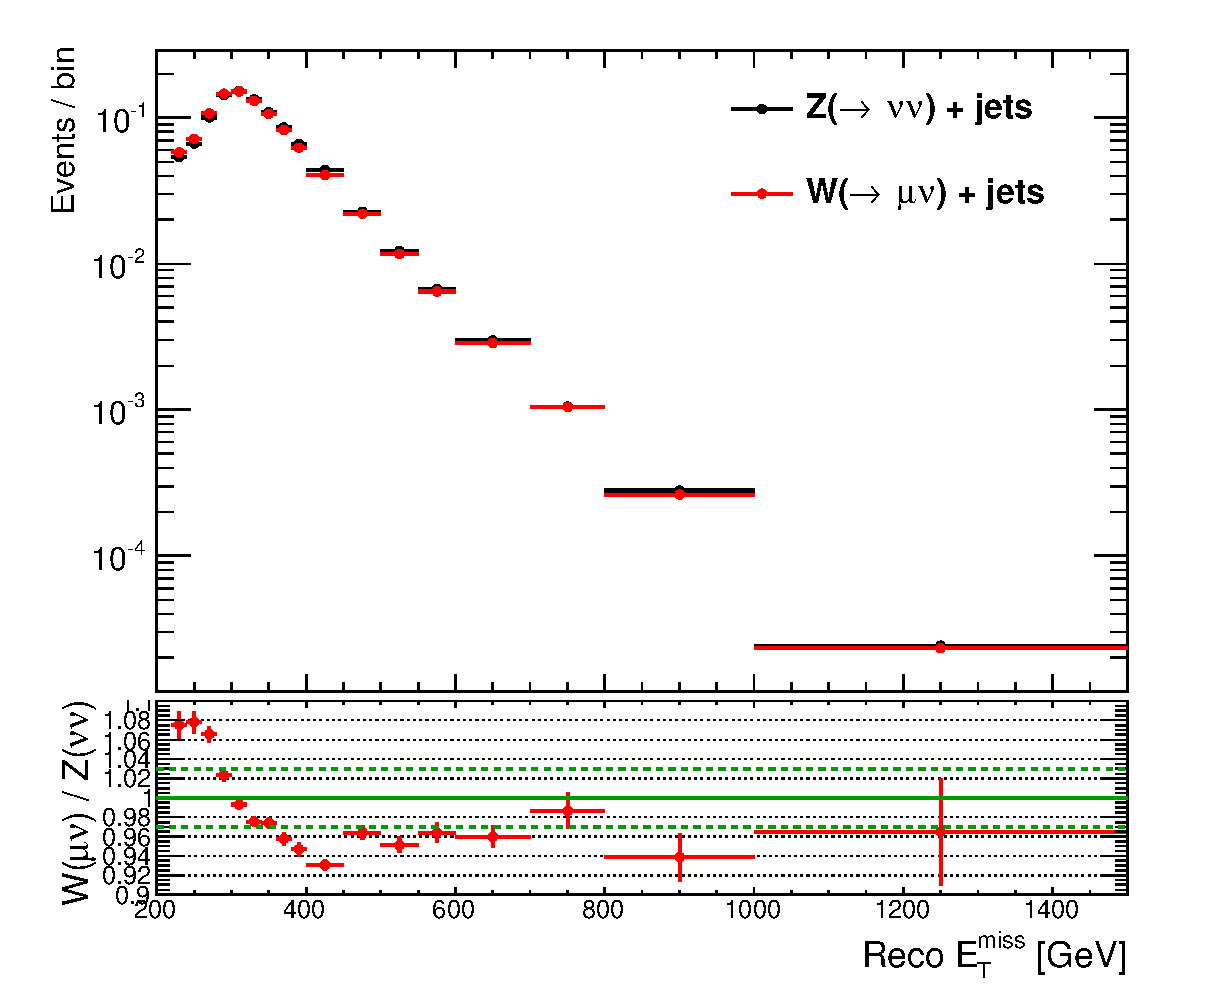
\includegraphics[width=0.49\textwidth]{Appendix_ClosureTestZnunu/Figures/compareNormalized_met_A6_Nom_CRcutsWZFiducialMu.eps}
  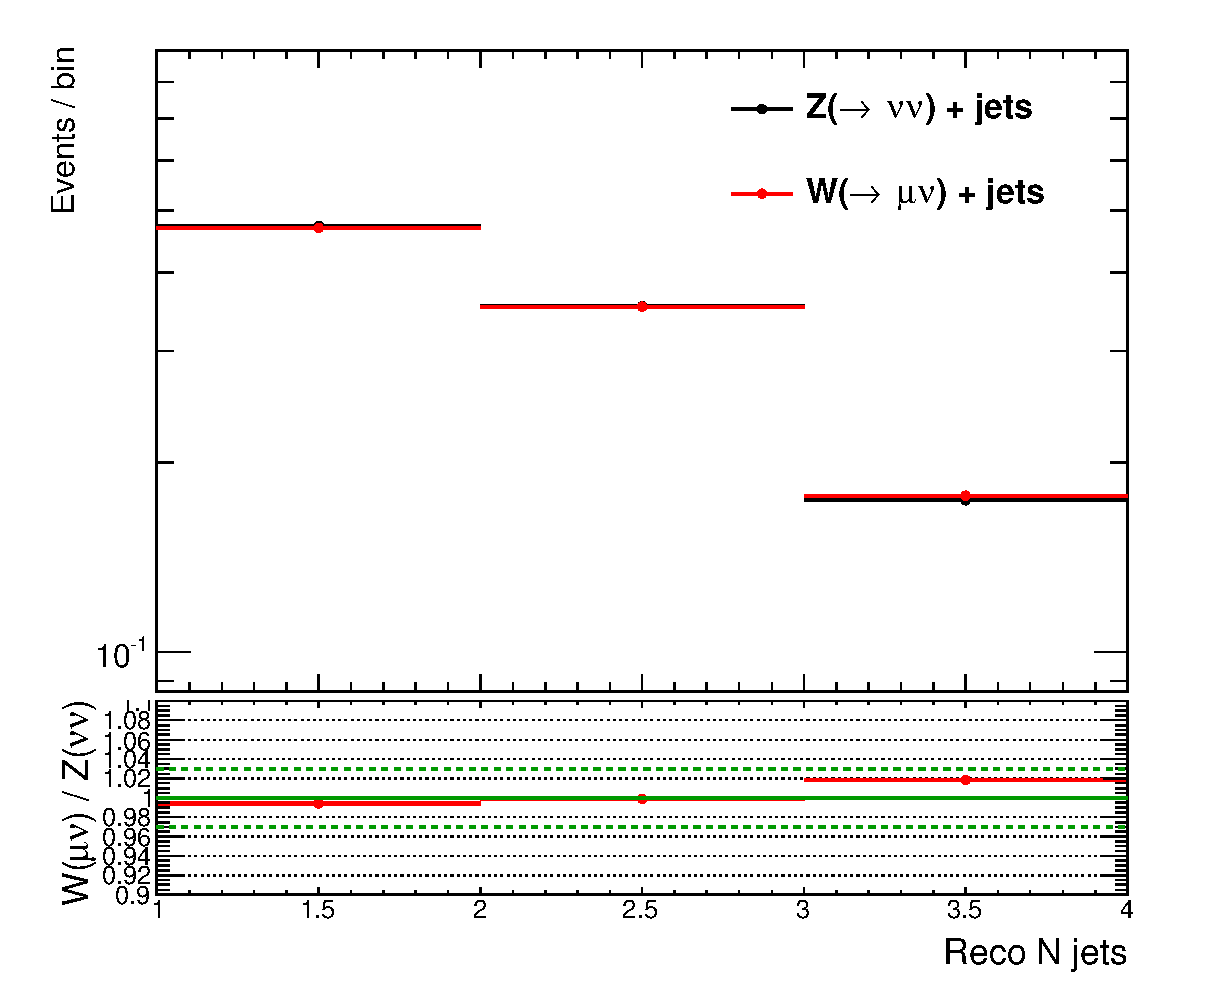
\includegraphics[width=0.49\textwidth]{Appendix_ClosureTestZnunu/Figures/compareNormalized_n_jets_A6_Nom_CRcutsWZFiducialMu.eps}
}                                                                          
\mbox{                                                                     
  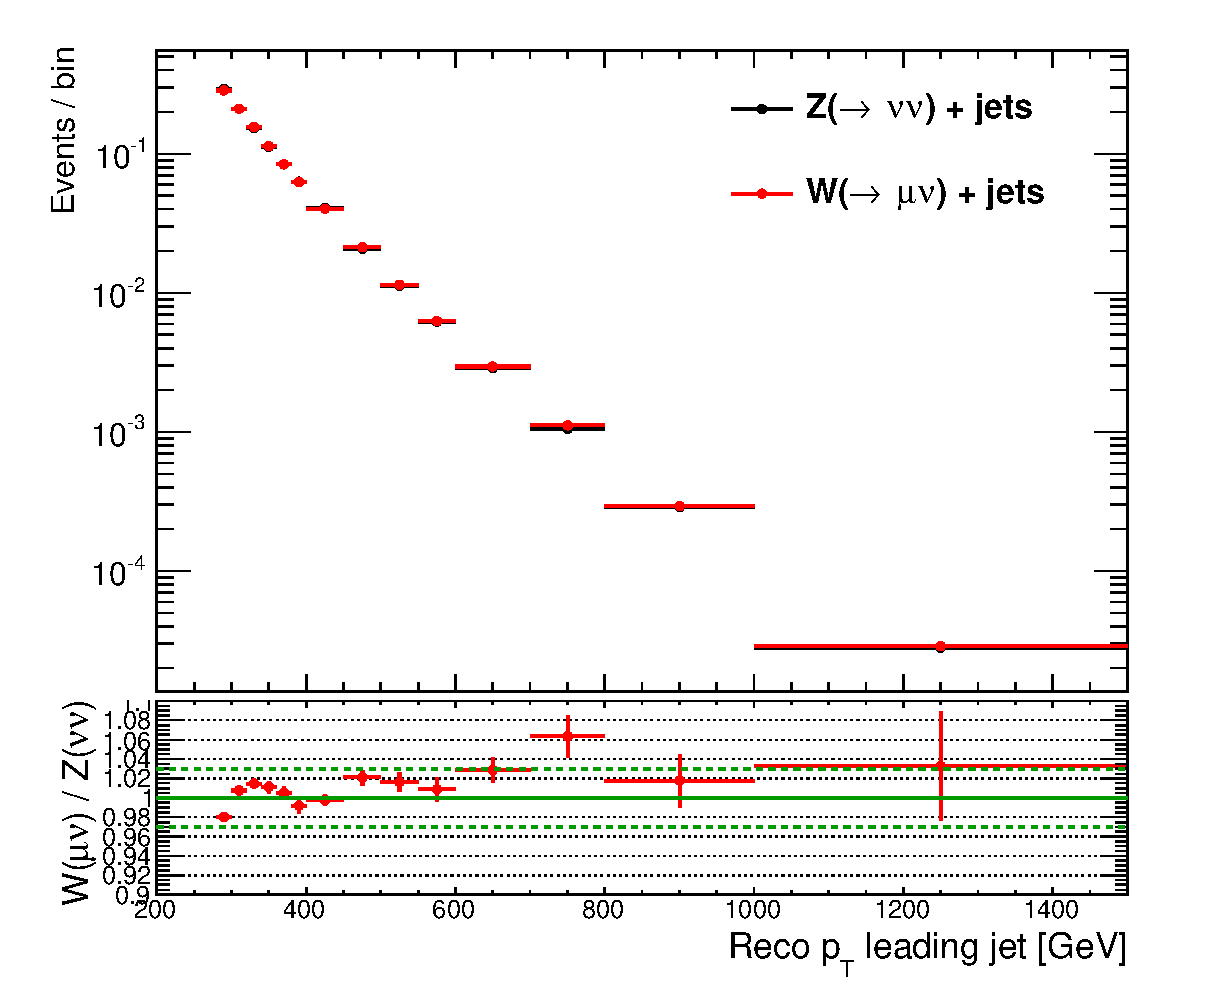
\includegraphics[width=0.49\textwidth]{Appendix_ClosureTestZnunu/Figures/compareNormalized_pt1_A6_Nom_CRcutsWZFiducialMu.eps}
  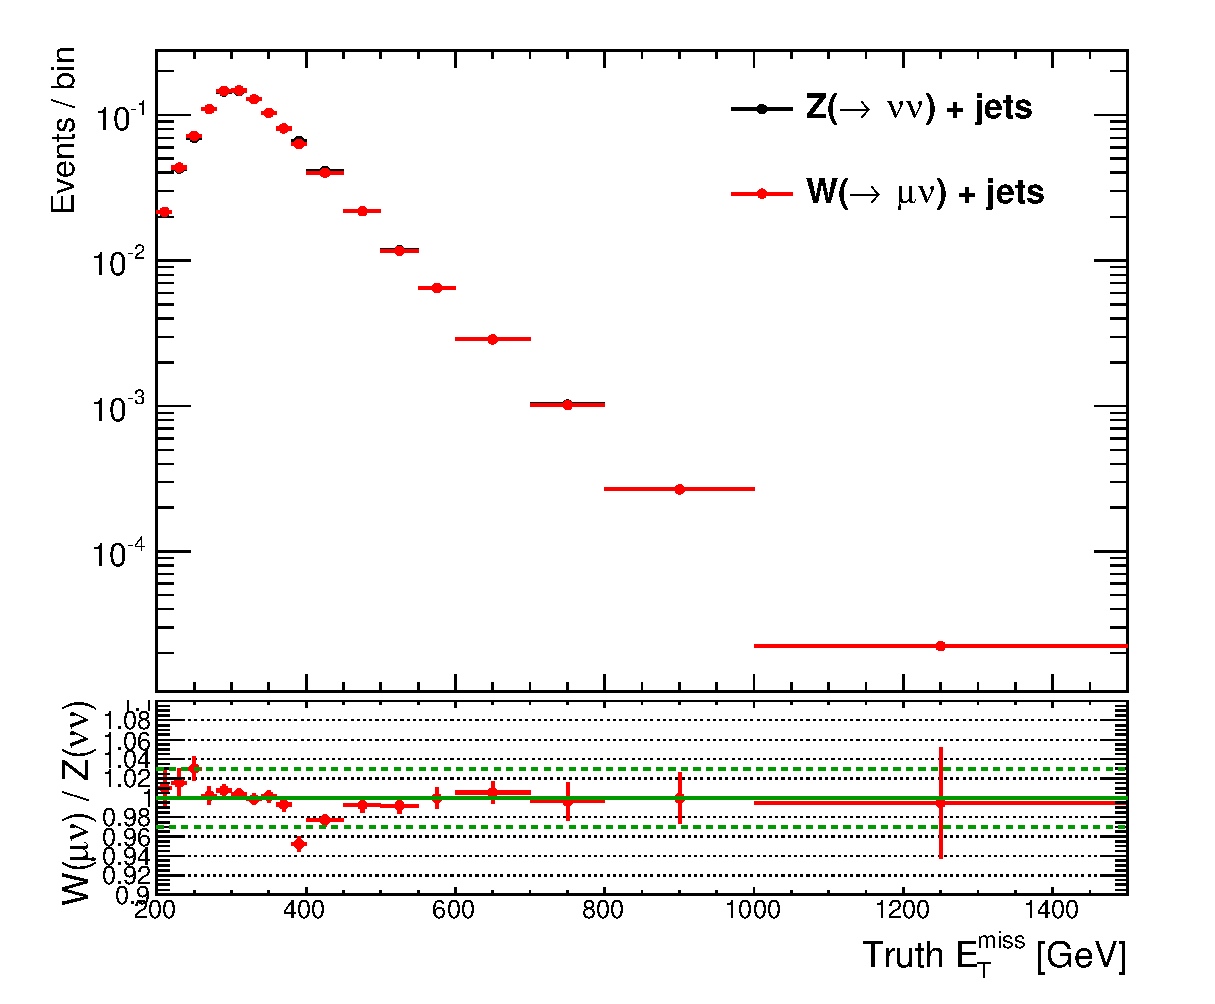
\includegraphics[width=0.49\textwidth]{Appendix_ClosureTestZnunu/Figures/compareNormalized_truth_met_A6_Nom_CRcutsWZFiducialMu.eps}
}
\end{center}
\caption[Comparison of different quantities in signal region M1 between $\wmn$+jets and $\znn$ MC simulations.
Comparisons are performed after applying a muon (pseudo muon) selection in the $\wmn$+jets ($\znn$) sample.]{Comparison of different quantities in signal region M1 between $\wmn$+jets and $\znn$ MC simulations.
Comparisons are performed after applying a muon (pseudo muon) selection in the $\wmn$+jets ($\znn$) sample.
}
\label{fig:closure8}
\end{figure}

Finally, Figure~\ref{fig:closey} compares the $\znn$ background prediction when it is normalized with the normalization factors extracted mainly from the $\wmn$+jets and $\zmm$+jets, for the signal regions M1 to M4.
The results are compatible within statistical uncertainties.

\begin{figure}
\begin{center}
\mbox{
  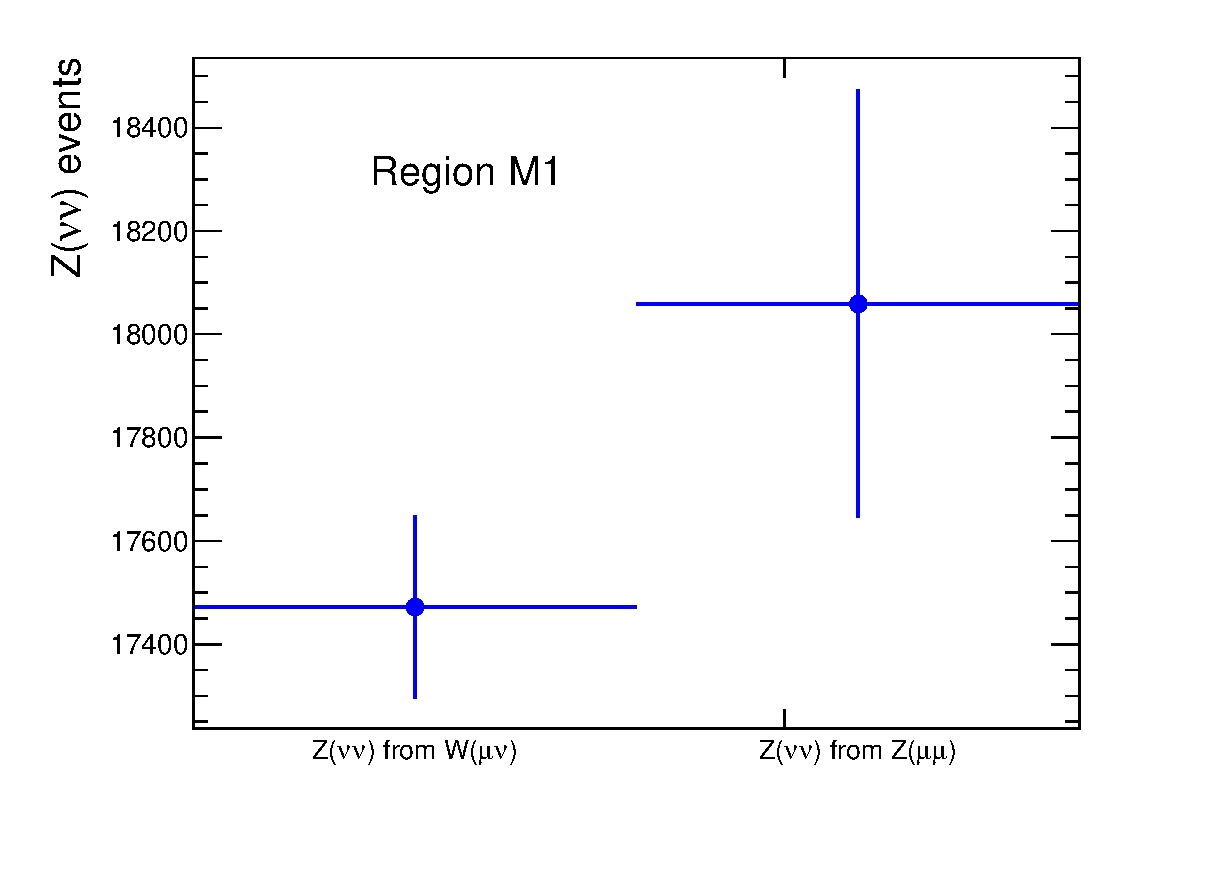
\includegraphics[width=0.49\textwidth]{Appendix_ClosureTestZnunu/Figures/CRwmn_vs_CRzmm_ZnunuEvents_A6.eps}
  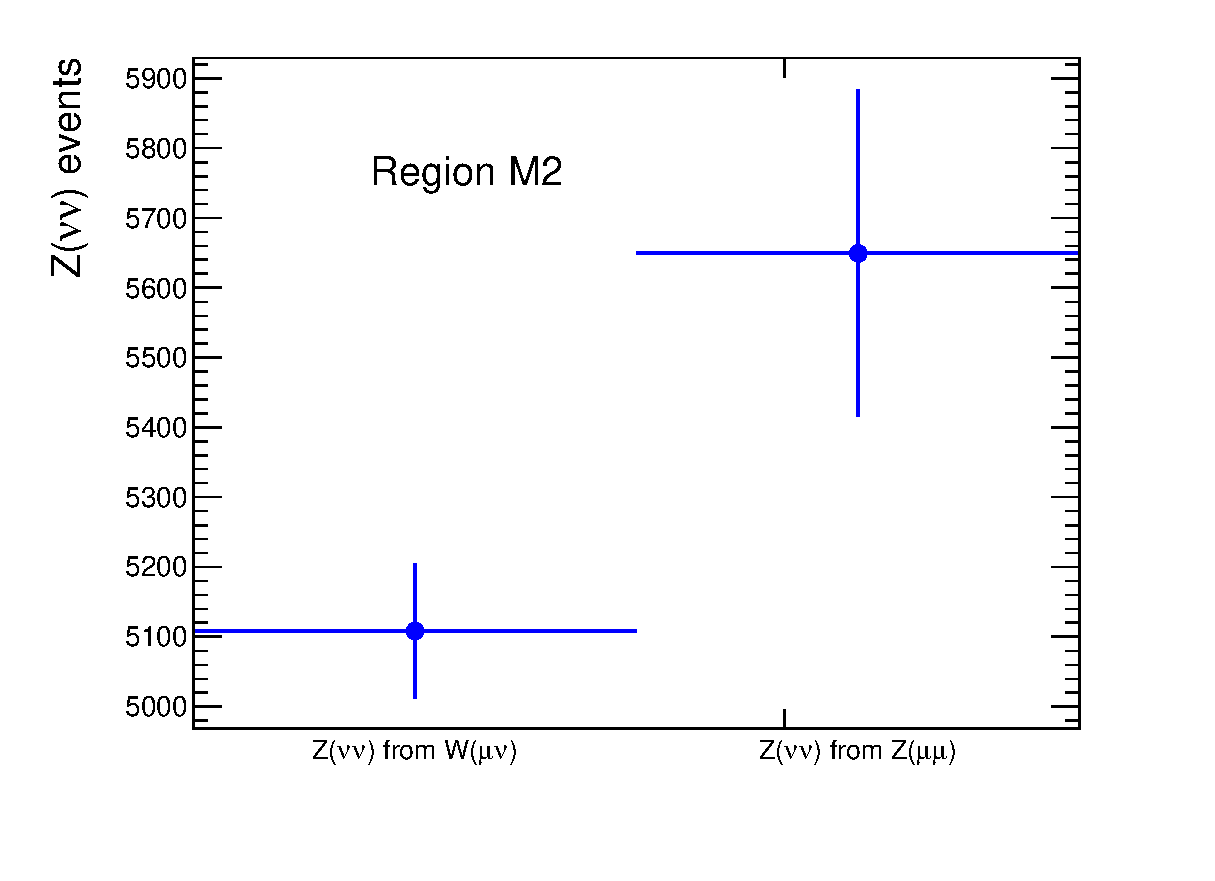
\includegraphics[width=0.49\textwidth]{Appendix_ClosureTestZnunu/Figures/CRwmn_vs_CRzmm_ZnunuEvents_A3.eps}
}                                                                         
\mbox{                                                                    
  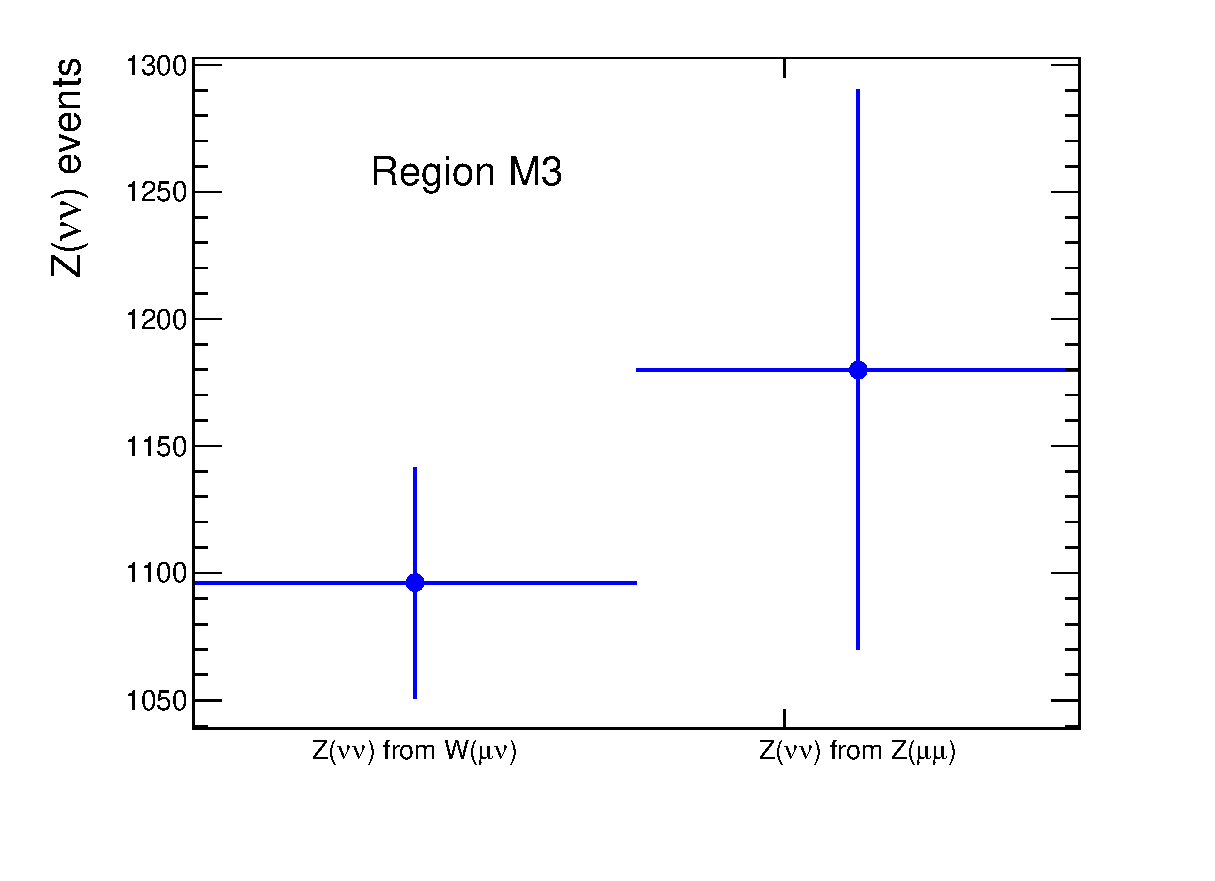
\includegraphics[width=0.49\textwidth]{Appendix_ClosureTestZnunu/Figures/CRwmn_vs_CRzmm_ZnunuEvents_A4.eps}
  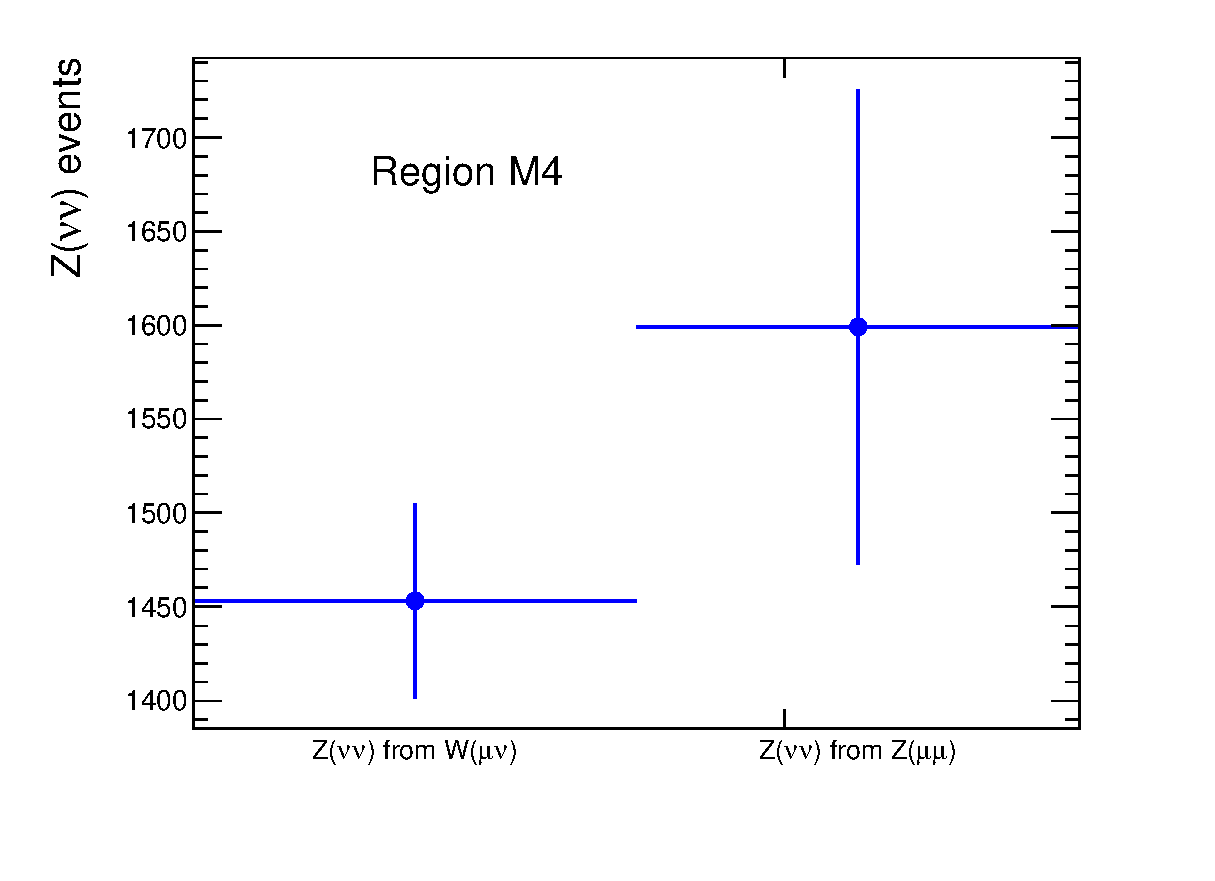
\includegraphics[width=0.49\textwidth]{Appendix_ClosureTestZnunu/Figures/CRwmn_vs_CRzmm_ZnunuEvents_A8.eps}
}
\end{center}
\caption{
Comparison of the $\znn$ contribution when is normalized with the same factor as the $\wmn$+jets or $Z/\gamma^{\ast}(\rightarrow \mu^{+}\mu^{-})$+jets processes. Only statistical uncertainties are presented.
}
\label{fig:closey}
\end{figure}

The effect of higher order electroweak corrections affecting differently the $W$ and the $Z$ production needs to be considered, as discussed in Refs.~\cite{Denner:2009gj,Denner:2011vu,Denner:2012ts}.
In order to properly account for this effect, the authors of the reference have been contacted and have provided the electroweak corrections in the $Z/W$ ratio for the selections M1 to M6.
The computed numbers are presented in Table~\ref{tab:ewkcorrTheorists}.
These higher order electroweak corrections are determined with a relatively large uncertainty dominated by the understanding of the photon induced processes~\cite{Denner:2009gj,Denner:2011vu,Denner:2012ts}.
In the analysis, no attempt is made to correct the $\znn$ estimation for this effect.
Instead, the difference is adopted as an additional systematic uncertainty, as shown in the Table.
This uncertainty varies from 2\% to 5\% as the leading jet $\pt$ and the $\met$ requirements tighten, which is added in quadrature to the 3\% uncertainty described above.

\begin{table}[!htb]
\begin{center}
\vspace*{1em}
\begin{tabular}{ccc}
\hline\hline
\multicolumn{3}{c}{{\bf EWK corrections at high $p_T$}} \\
\textbf{\phantom{00}SR\phantom{00}} & \textbf{EWK correction} & \textbf{syst. uncert.}            \\
\hline
%%
M1 & $\left(1.4 ^{+2.0}_{-1.8}\right)$\% & 2\%\\ [0.5ex]  
M2 & $\left(1.5  ^{+2.3}_{-2.6}\right)$\% & 2\%\\ [0.5ex] 
M3 & $\left(2.6  ^{+2.3}_{-3.5}\right)$\%& 3\% \\ [0.5ex] 
M4 & $\left(3.6 ^{+2.3}_{-3.5}\right)$\%& 4\% \\[0.5ex]   
M5 & $\left(3.7 ^{+2.9}_{-4.6}\right)$\%& 4\% \\[0.5ex]   
M6 & $\left(5.1 ^{+3.6}_{-5.5}\right)$\% & 5\%\\ [0.5ex] \hline\hline
\end{tabular}
\end{center}
\caption[Uncertainty adopted on the $\znn$ estimation associated to higher order electroweak radiative corrections with the $W/Z$ ratio.]
{Electroweak higher-order corrections on the $W/Z$ ratio and the associated systematic uncertainty applied to the $\znn$ background contribution.}
\label{tab:ewkcorrTheorists}
\end{table}
